\chapter{Literature Survey}
\section{Cycle Shrinking Algorithm}

Cycle shrinking algorithm~\cite{cycle1} allows loops with cyclic data dependencies to be partially parallelized when the dependence distances are known. Minimum distance between source and sink for a dependence is known as dependence distance. This is a vector for nested loops. \\

The idea of cycle shrinking has been extended in three ways: \\
\begin{enumerate}
\item {\bf Simple shrinking}: Minimum dependence distance for each nest level is calculated separately and then partitions are created based in these values. 
\item {\bf Selective shrinking}: Outermost level with positive dependence distance is selected and then simple shrinking is applied only at this level. All lower level loops are done in parallel. 
\item {\bf True distance shrinking}: The partition is made based on the actual number of iterations between the source and the sink ("true distance") of the dependencies considering the loop bounds at each nest level. 
\end{enumerate}

\subsection{Example}
Consider the following example: \\
DO I = 0 to 9 \\
\indent DO J = 0 to 9 \\
\indent \indent A[I+3, J+4] = B[I, J] \\
\indent \indent B[I+2, J+3] = A[I, J] \\
\indent ENDO \\
ENDO \\

The two dependence distances are (3, 4) and (2, 3). The partitions created by cycle shrinking algorithm are shown in the figure~\ref{fig:cycle_shrinking_example}. \\


\begin{figure}
\centering
\begin{subfigure}{0.45\textwidth}
  \centering
  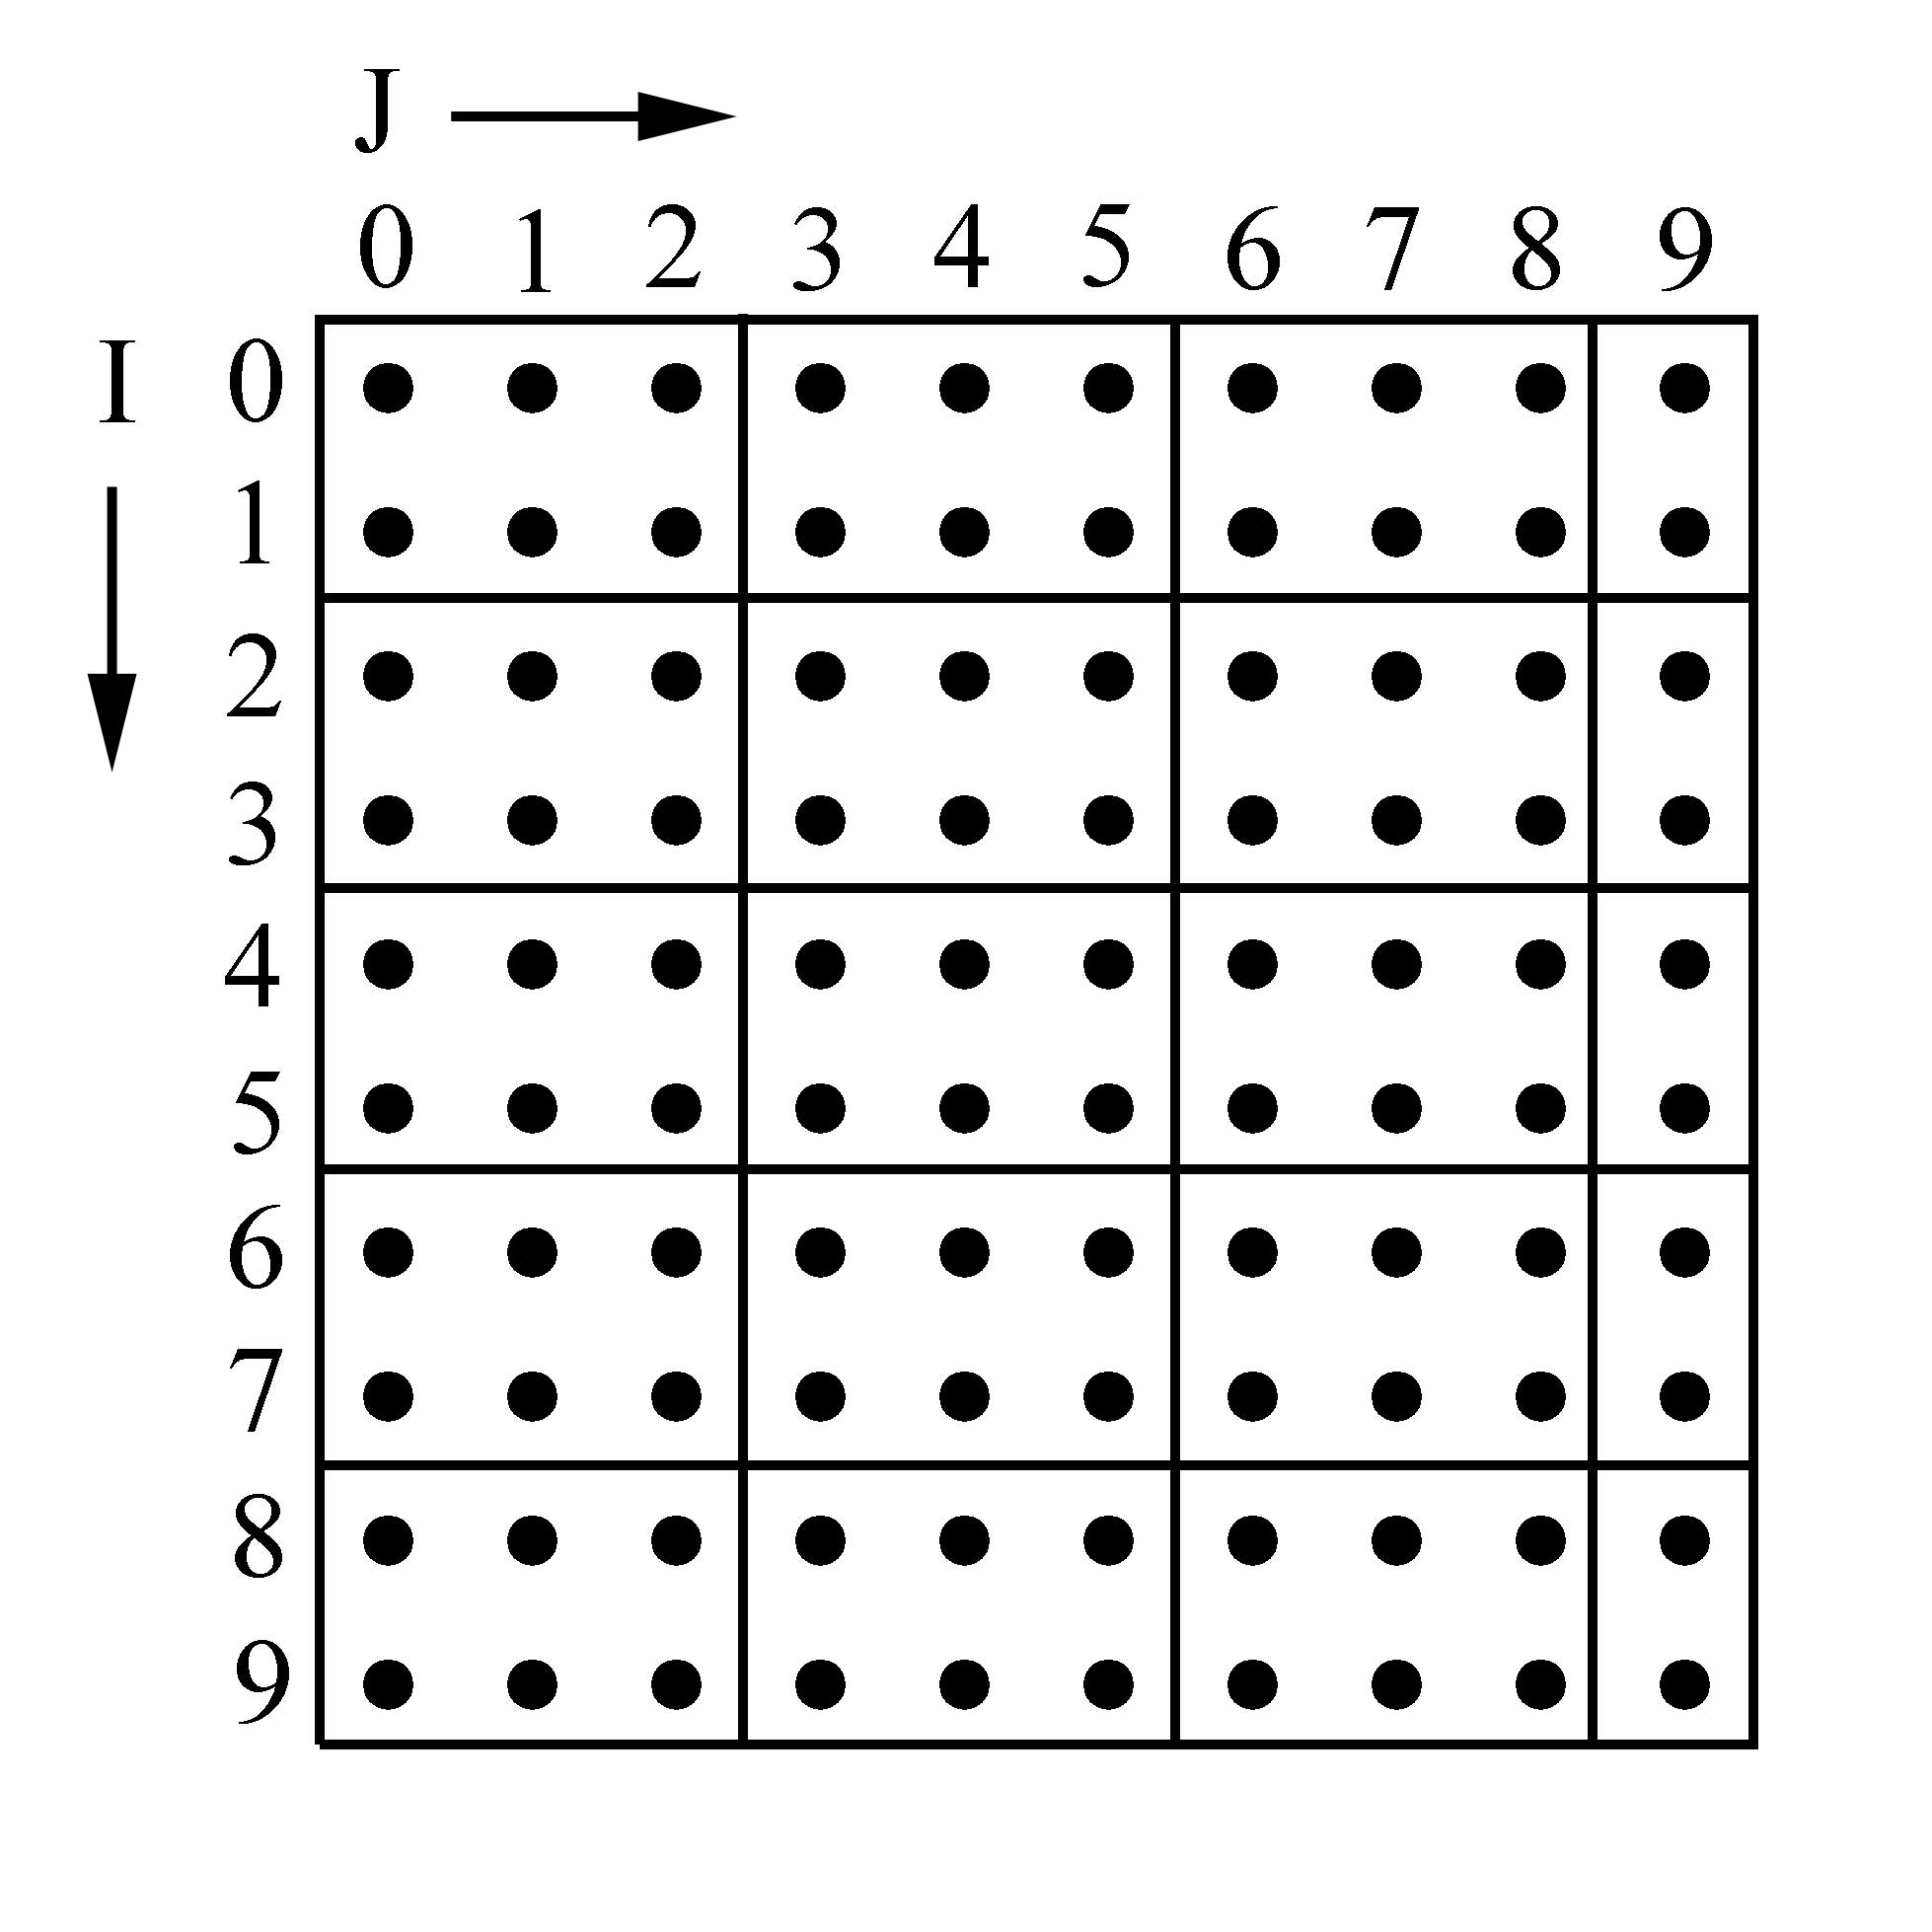
\includegraphics[width=\textwidth]{Figures/simple.jpg}
  \caption{}
  \label{fig:simple}
\end{subfigure} 
\begin{subfigure}{0.45\textwidth}
  \centering
  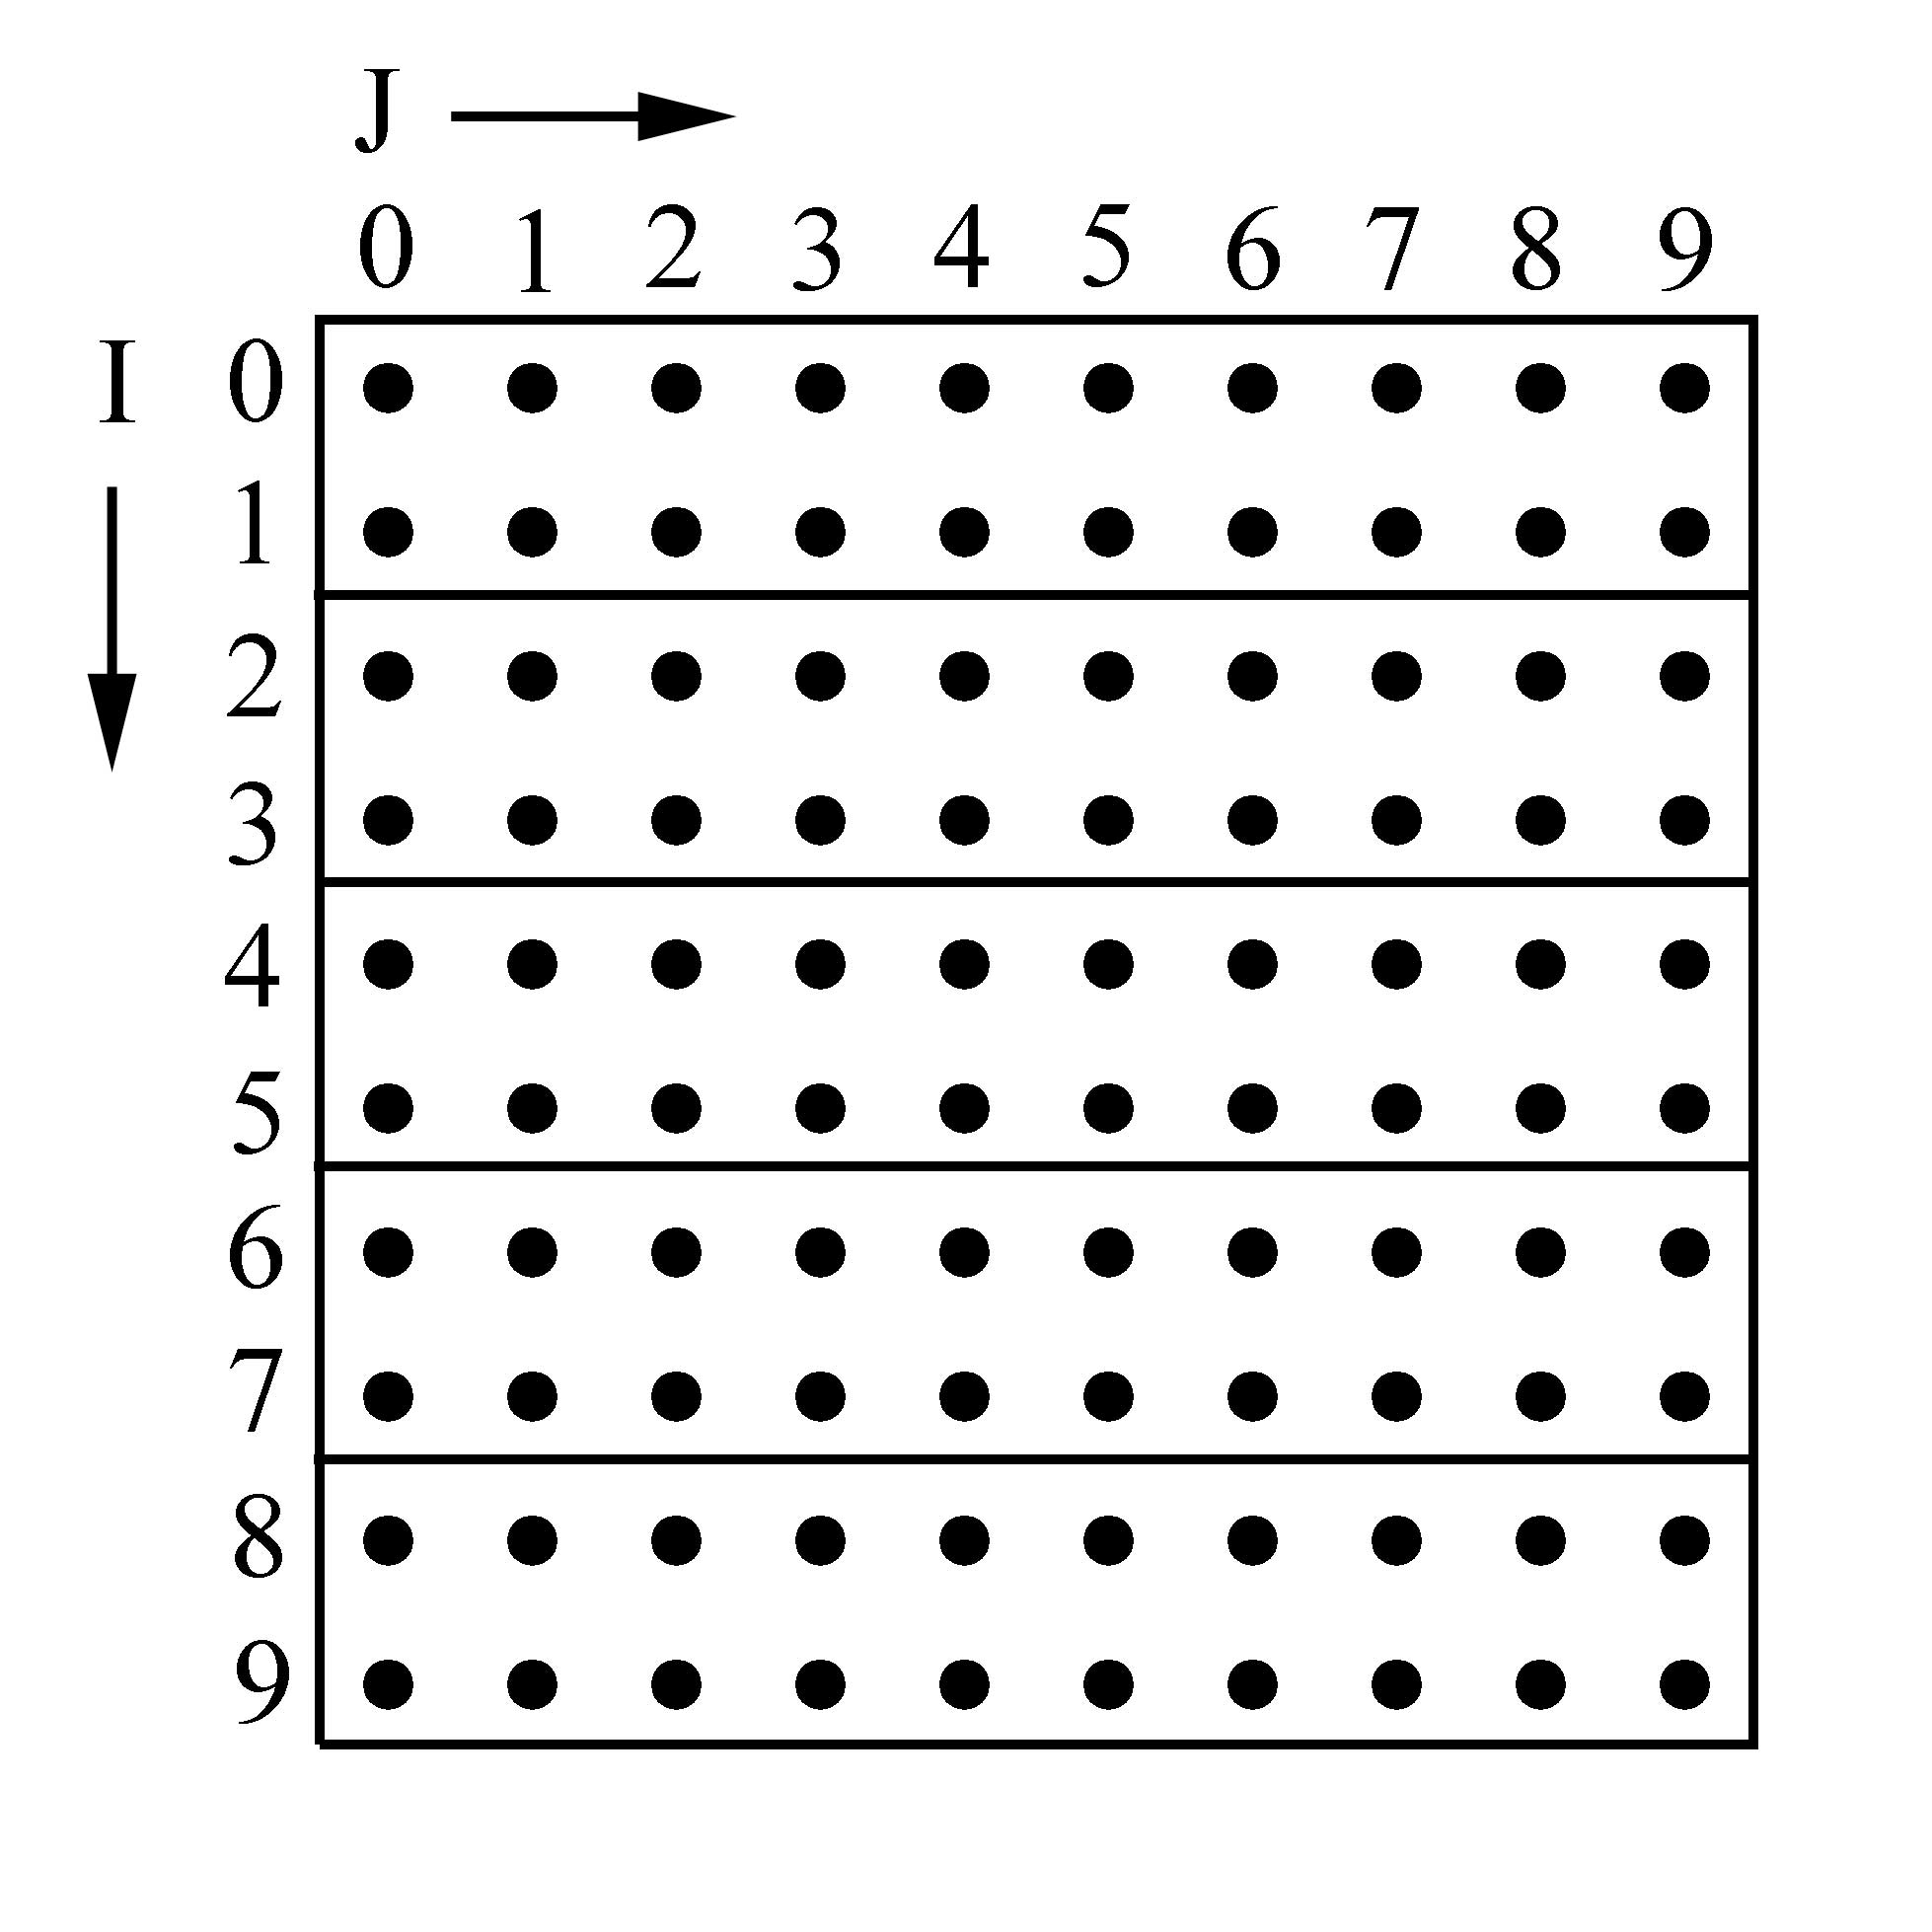
\includegraphics[width=\textwidth]{Figures/selective.jpg}
  \caption{}
  \label{fig:selective}
\end{subfigure}  \\
\begin{subfigure}{0.45\textwidth}
  \centering
  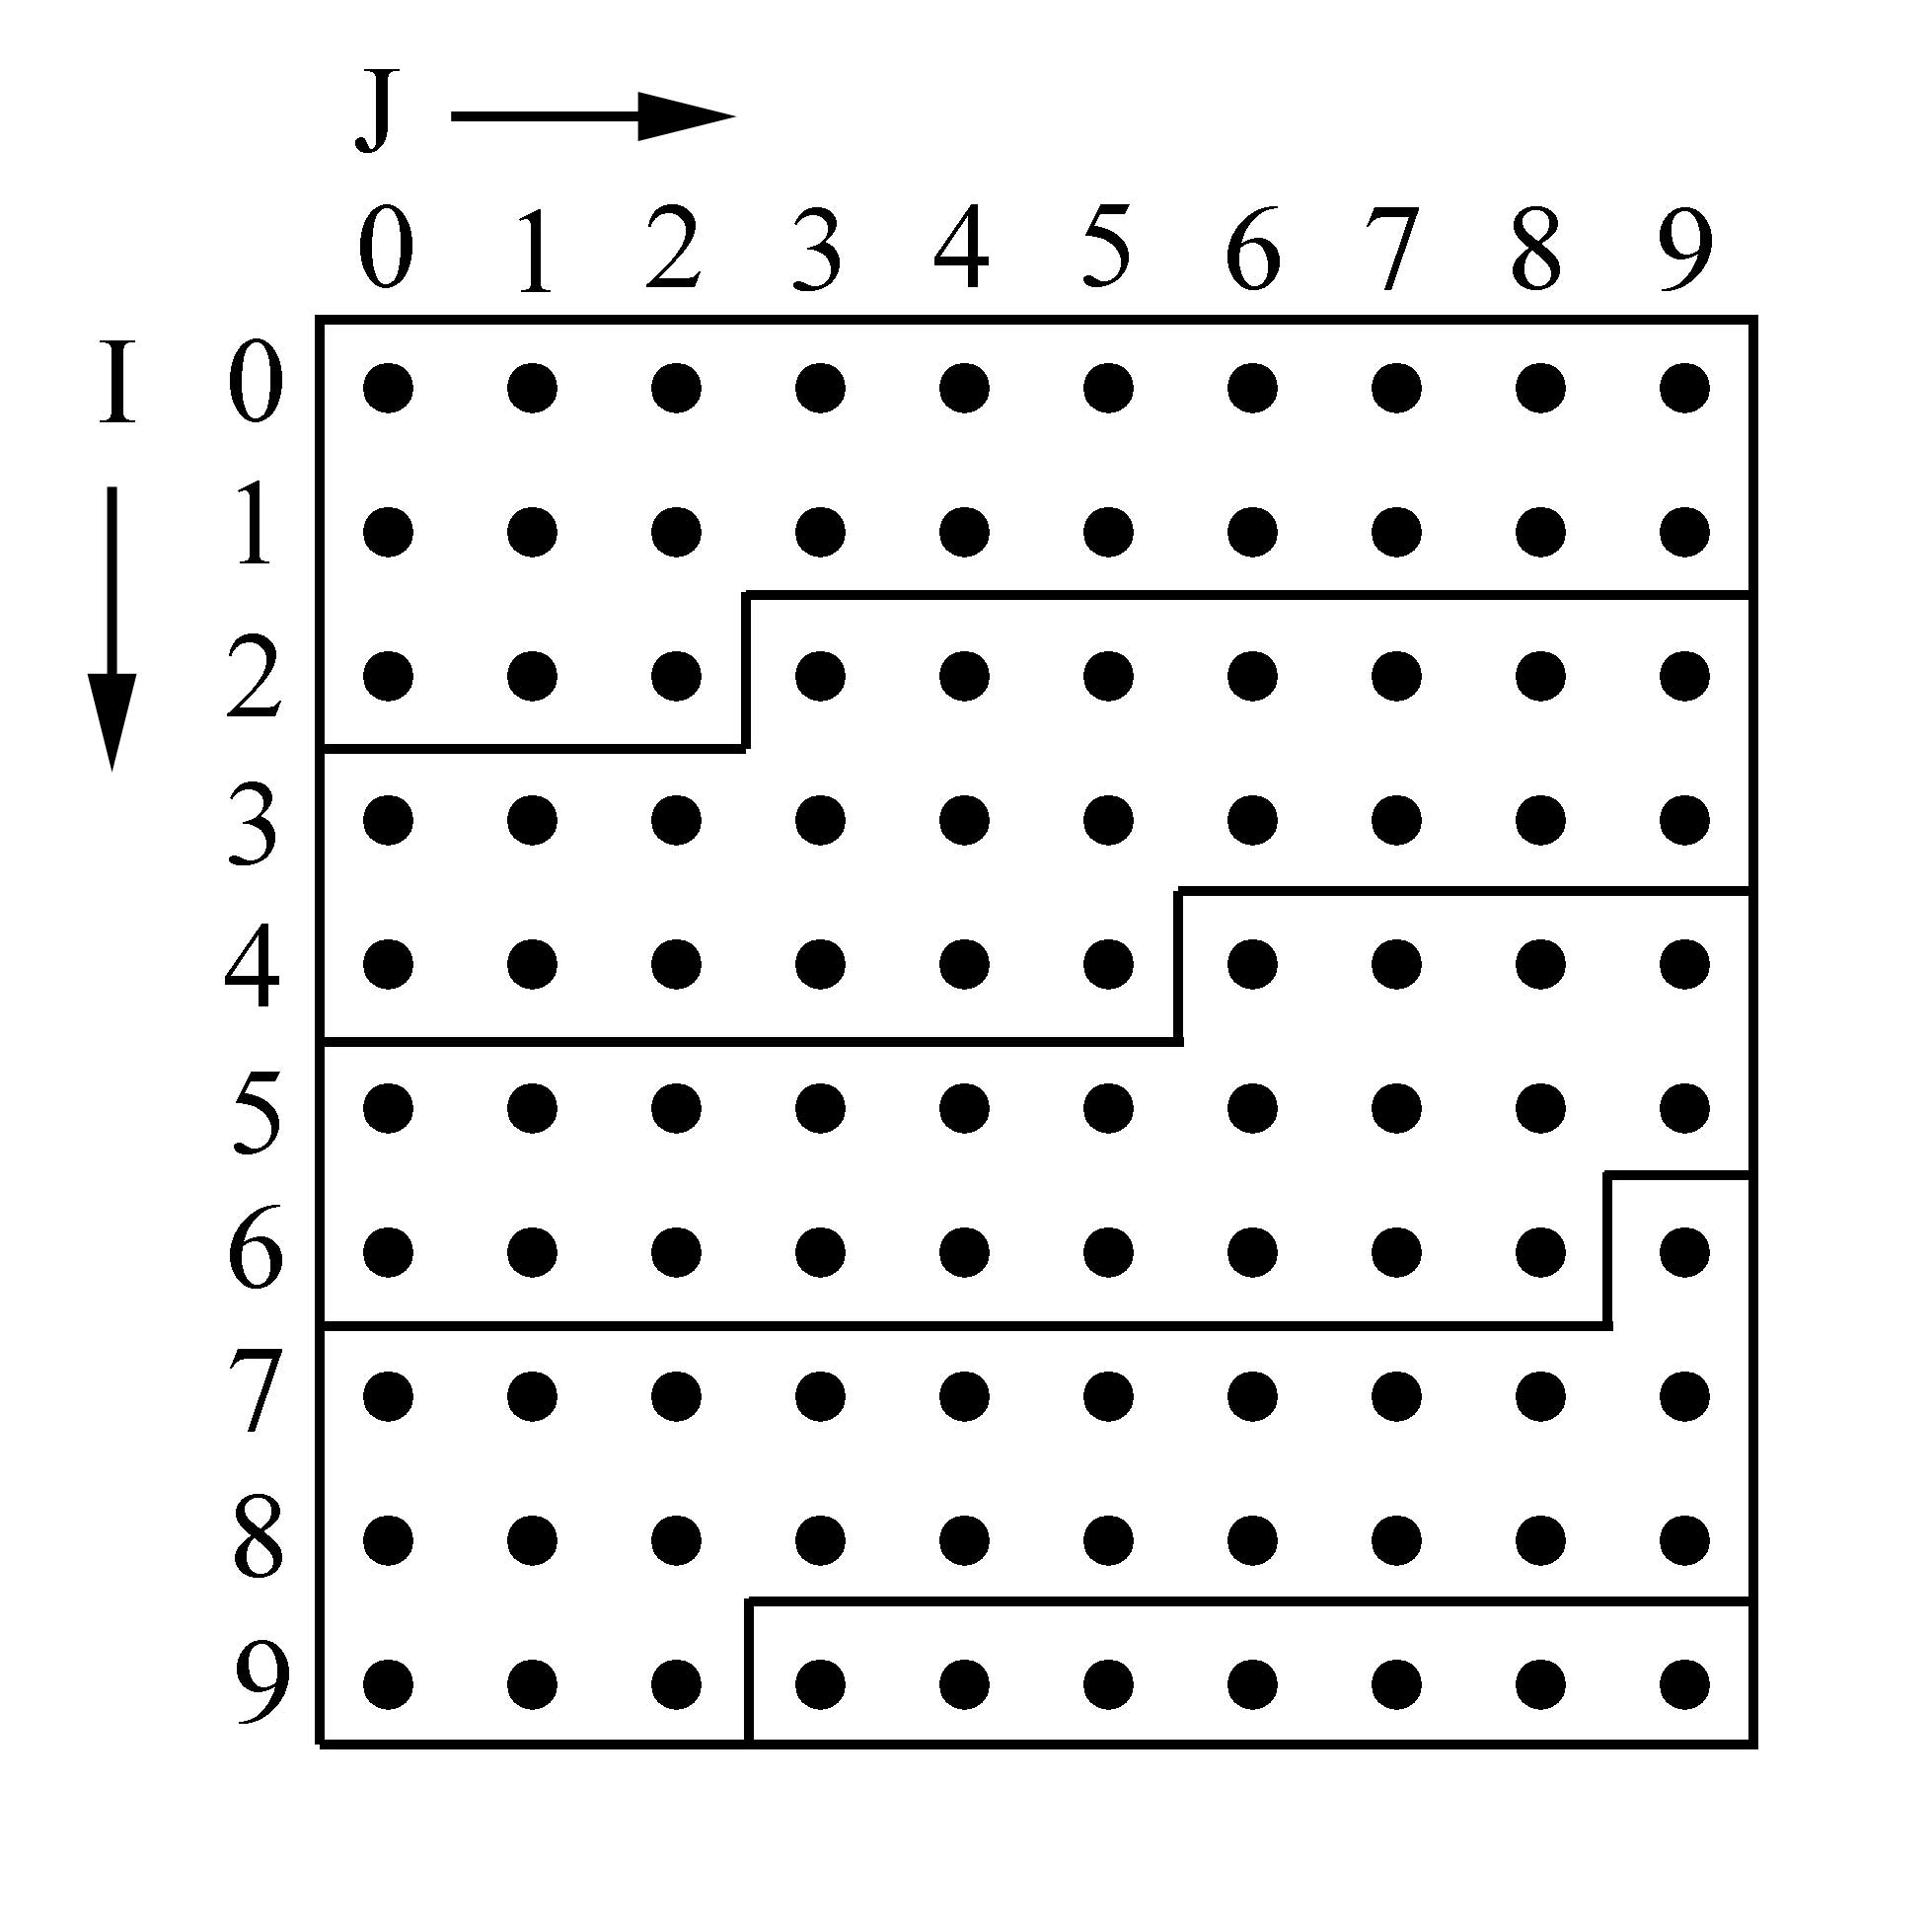
\includegraphics[width=\textwidth]{Figures/true_distance.jpg}
  \caption{}
  \label{fig:true_distance}
\end{subfigure}
\begin{subfigure}{0.45\textwidth}
  \centering
  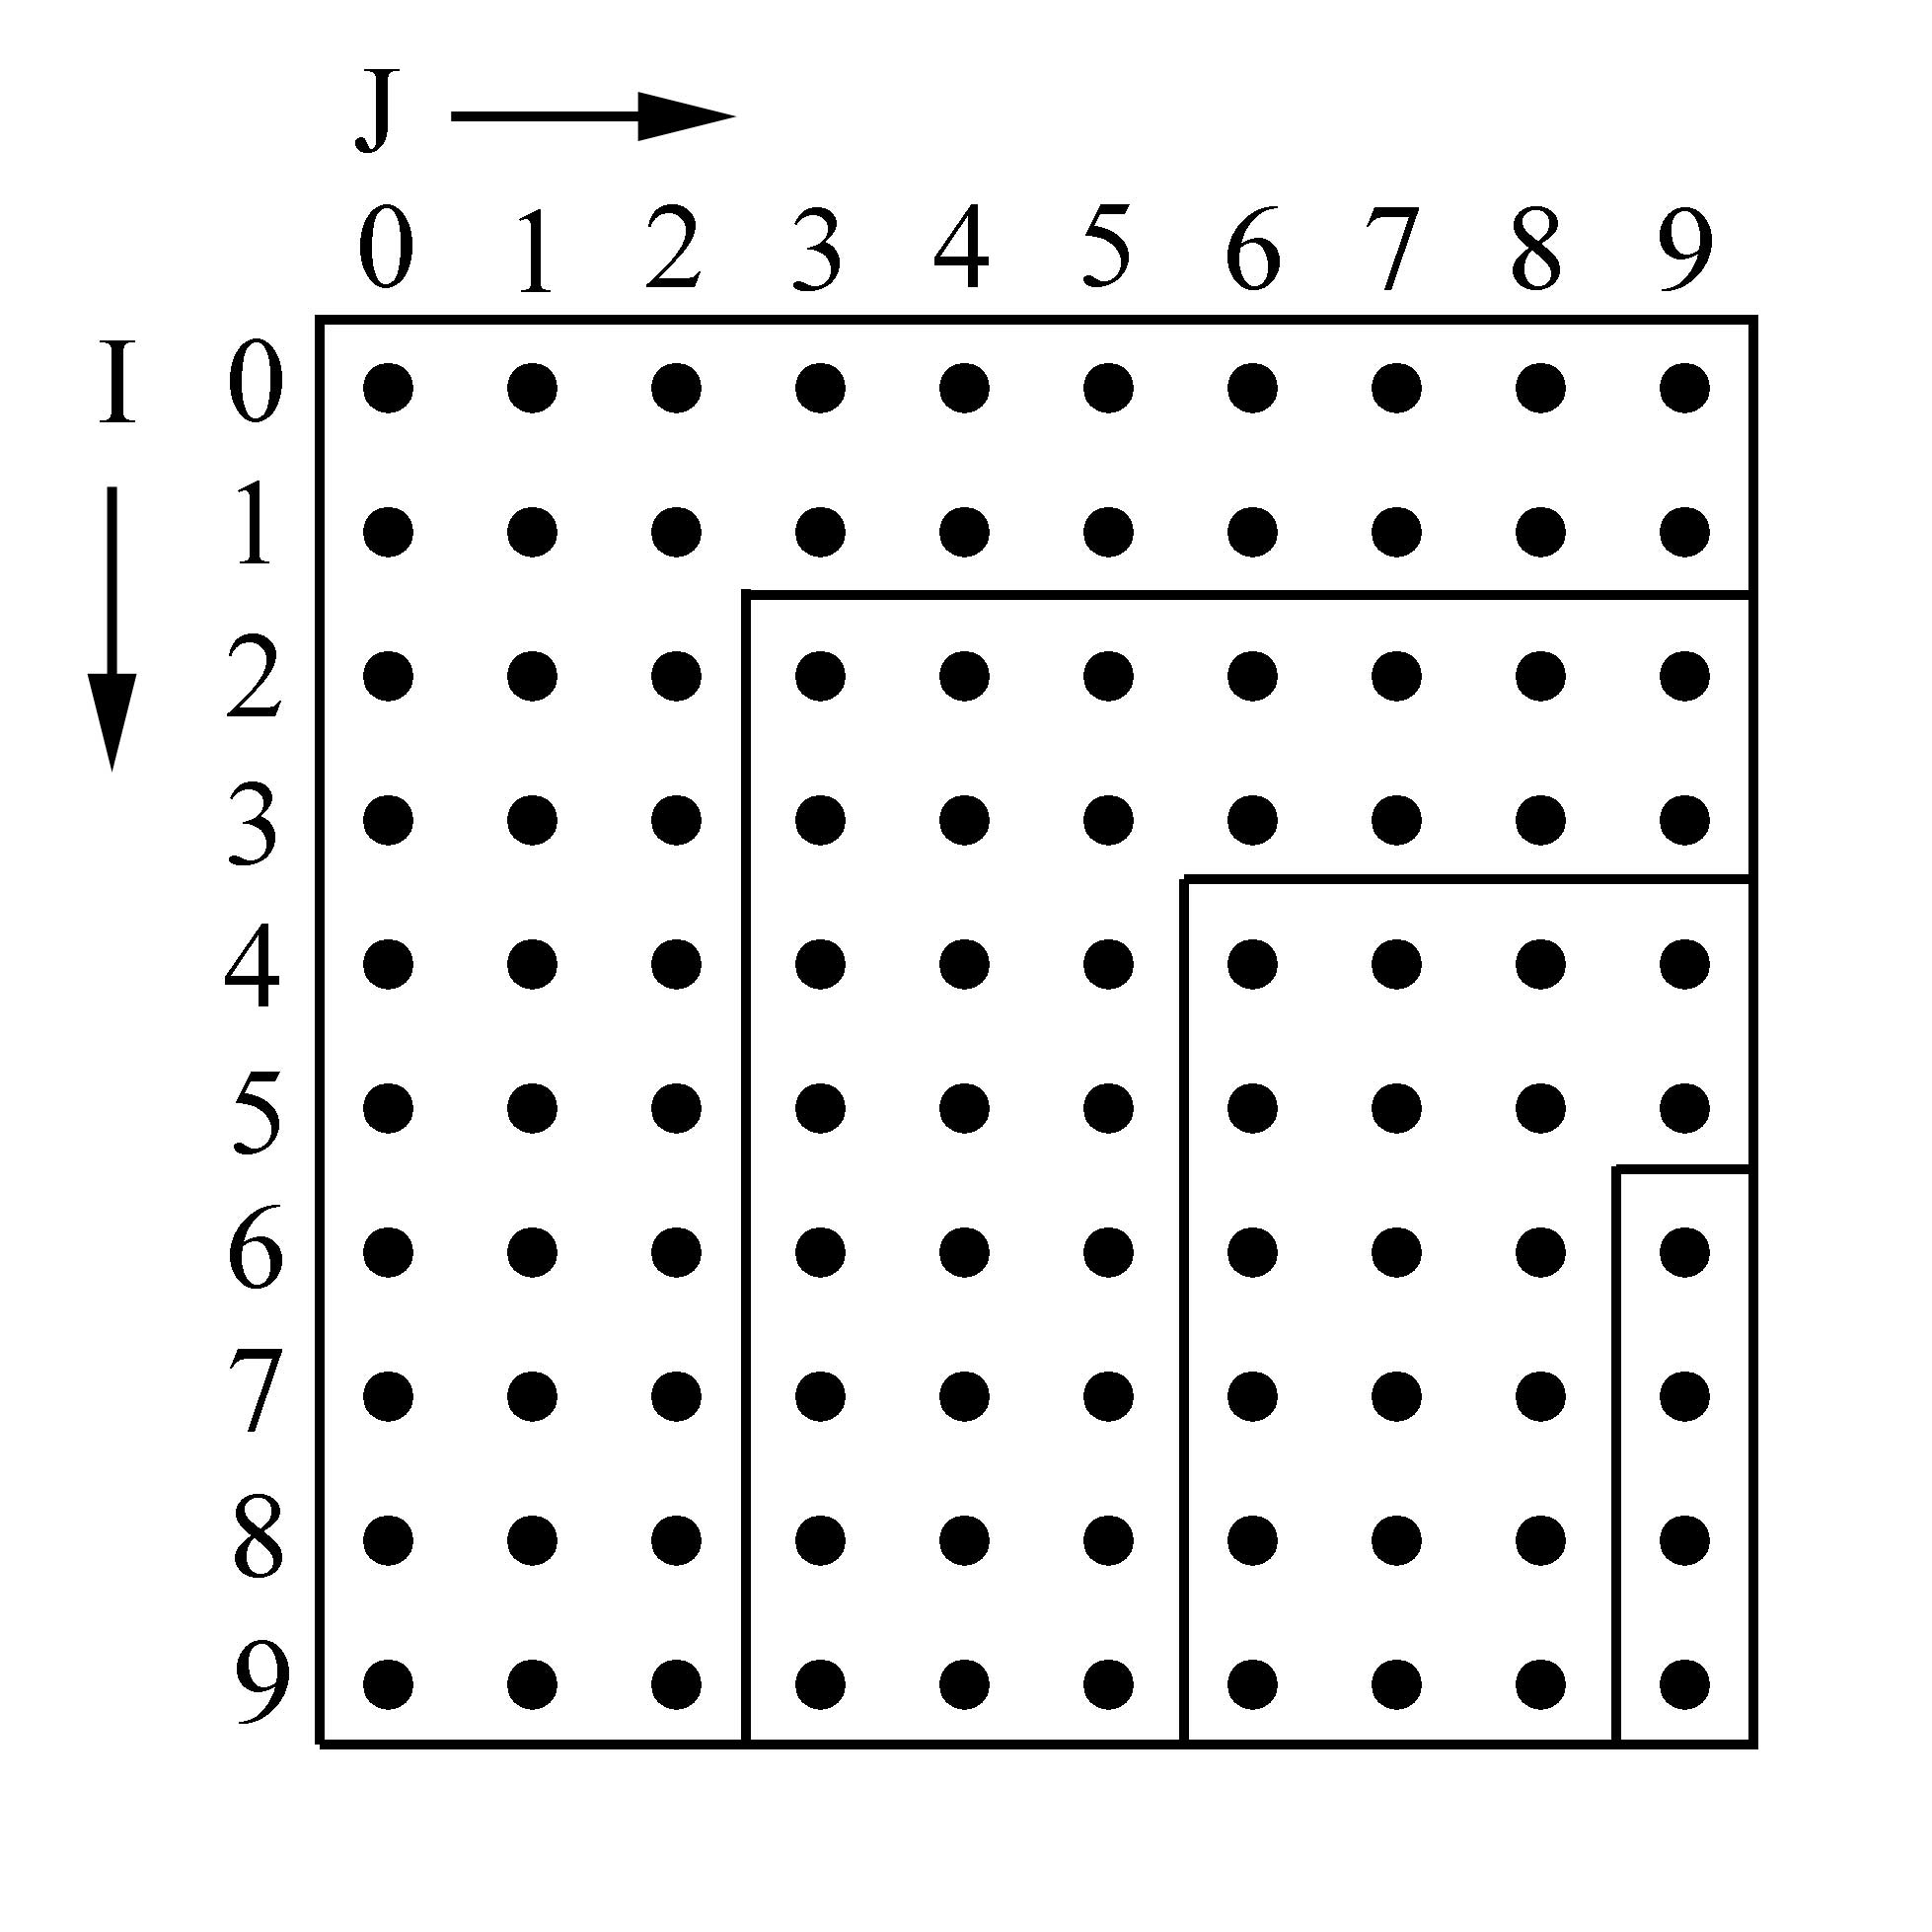
\includegraphics[width=\textwidth]{Figures/extended.jpg}
  \caption{}
  \label{fig:extended}
\end{subfigure}
\caption{(a) Partitions by simple shrinking. (b) Partitions by selective shrinking. (c) Partitions by true distance shrinking. (d) Partitions by extended cycle shrinking algorithm}
\label{fig:cycle_shrinking_example}
\end{figure}

However, a greater degree of parallelism can be achieved if the partitions are made as shown in the figure~\ref{fig:extended}. It reduces the number of partitions.
Extended cycle shrinking algorithm creates paritions in this manner. \\


\section{Extended Cycle Shrinking Algorithm}

Extended Cycle Shrinking Algorithm~\cite{extended} has two cases, when there are only constant dependence distances and when there are variable dependence distances. \\

\subsection{Constant Dependence Distances}

If two array accesses have a dependence among them then they are called as a reference pair.
Consider the case where all the reference pairs have only constant dependence distances. The dependence distance vector of a reference pair R is denoted as $\Phi(R)$ and $k^{th}$ component of the dependence distance $\Phi(R)$ is denoted as $\Phi_{k}(R)$. Then we define the dependence distance of vector of loop L denoted by $\Phi(L)$ as given below: \\

For each nest k of the loop, 
\begin{itemize}
\item $\Phi_k(L) = 0$ if there exists some reference pair R for which $\Phi_k(R) = 0$, or there exist two reference pairs R and R' such that $\Phi_k(R)$ and $\Phi_k(R')$ have opposite signs. 
\item $\Phi_k(L) = min(|\Phi_k(R)|)$ if sign($\Phi_k(R)$) is positive for all R, and
\item $\Phi_k(L) = -min(|\Phi_k(R)|)$ otherwise.
\end{itemize}

The partitions are created using $\Phi(L)$. The $k^{th}$ coordinate of the $i^{th}$ apex point of the partition is $(i-1)*\Phi_k(L)$ if $\Phi_k(L) > 0$, otherwise the apex point for that index is calculated from the other end of loop bound and the direction of partition is also opposite. \\

For example of figure~\ref{fig:extended}, \\
$\Phi(L) = (2, 3)$ \\
Therefore the apex points are (0, 0), (2, 3), (4, 6) and (6, 9). \\

\subsection{Variable Dependence Distances}

In the case of variable dependence distances, only those cases are considered where each source can have only one sink for a given reference pair. Unlike in the constant dependence distance case, here the dependence distances vary with the loop indices. Dependence distance is function of loop indices in this case. Thus, instead of summarizing the dependence for the entire loop, the summarization is done at each apex. \\

\begin{figure}
\caption{Variable dependence distances}
\label{fig:variable1}
\centering 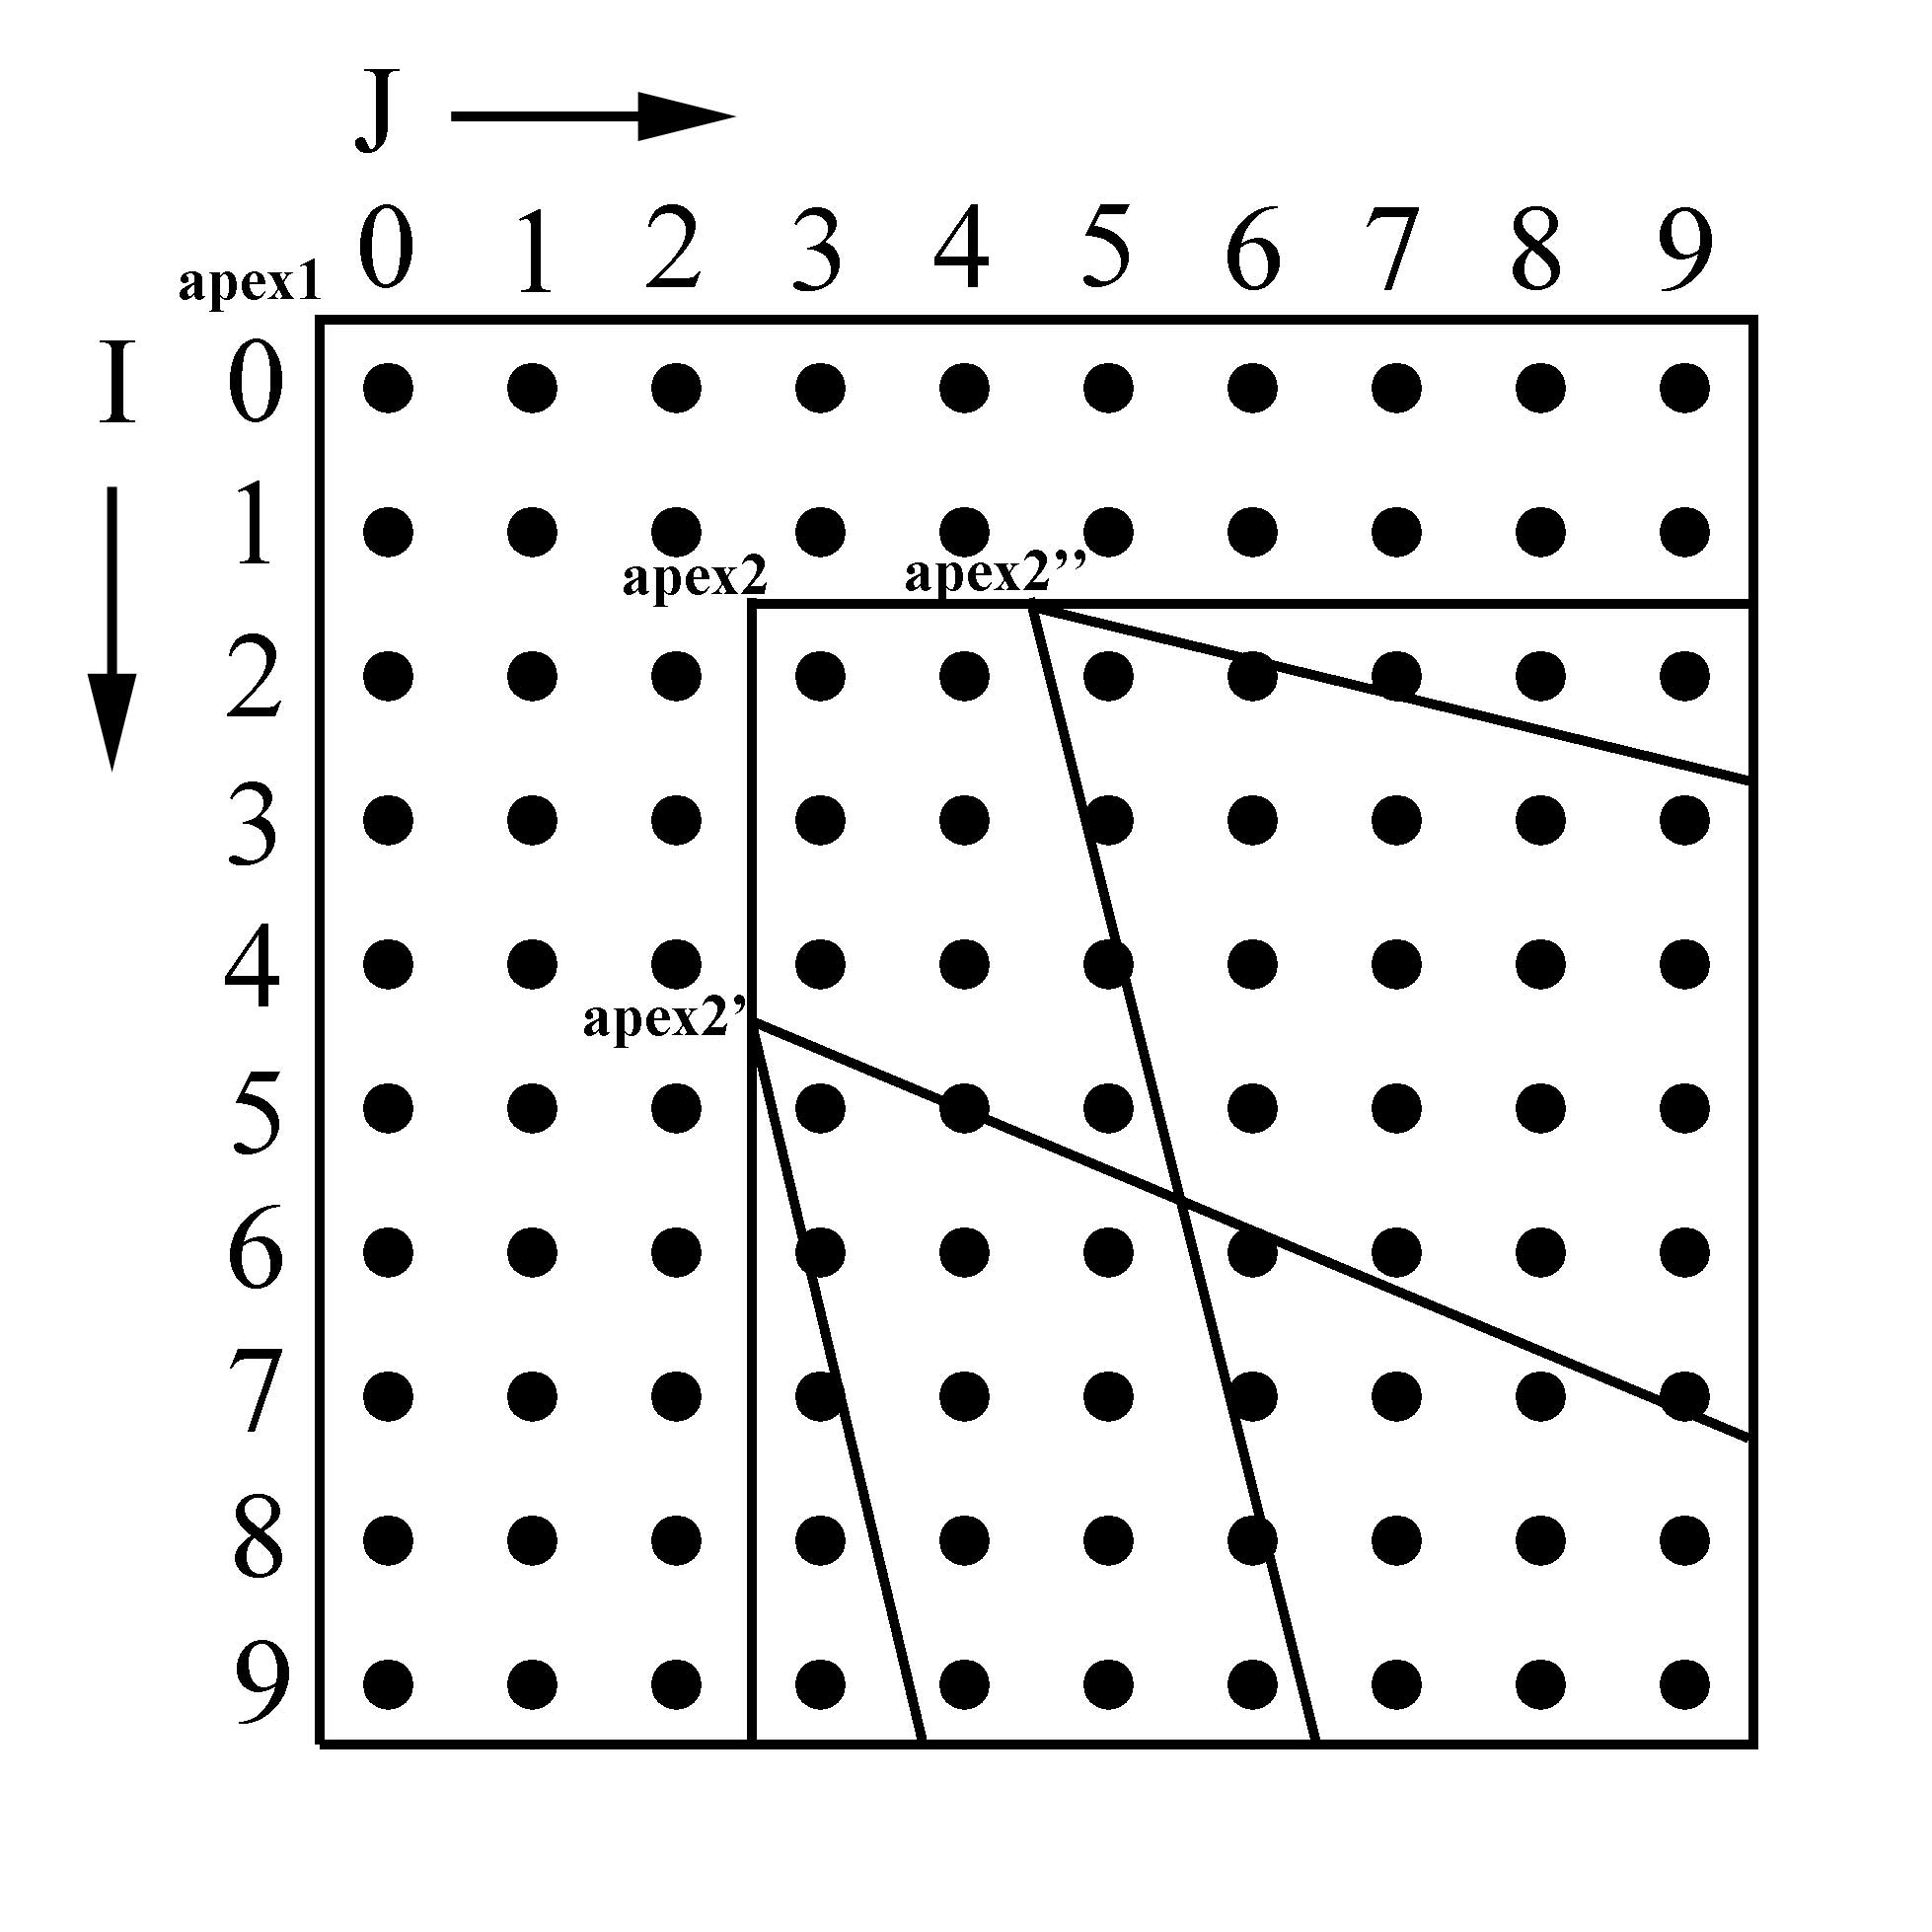
\includegraphics[width=0.7\textwidth]{Figures/variable1.jpg}
\end{figure}

As shown in the figure~\ref{fig:variable1}, apex1 is the initial apex point. We obtain apex2' and apex2'' as sinks of apex1. Then the sinks of all sources inside the cone of apex1 lie inside the cones formed by apex2' and apex2''. We summarize these two apexes to obtain apex2 as the next apex point in the partition. This procedure is repeated to obtain subsequent apex points. Once the apex points are known, the partitions are created in similar way as was done in the constant dependence distance case. \\



\noindent Consider the following example: \\
DO I = 0 to 9 \\
\indent DO J = 0 to 9 \\
\indent \indent A[2I+J+3, I+4J+2] = B[I+3, J+3] \\
\indent \indent B[3I+J+4, 2I+2J+3] = A[I+1, J+1] \\
\indent ENDO \\
ENDO \\

\noindent Dependence distances are : \{(I+J+2, I+3J+1), (2I+J+1, 2I+J)\} \\

\noindent apex1 = (0, 0)\\
Dependence distances: \{(2, 1), (1, 0)\}\\
Summarized dependence distance = (1, 0)\\
apex2 = (1, 0)\\

\noindent Dependence distances: \{(3, 2), (3, 2)\}\\
Summarized dependence distance = (3, 2)\\
apex3 = (4, 2)\\

\noindent Dependence distances: \{(8, 11), (11, 10)\}\\
Summarized dependence distance = (8, 10)\\
apex4 = (12, 12) which is out of range and thus all partitions have been found\\

The partitions generated from this example are shown in the figure~\ref{fig:variable_eg}
\begin{figure}
\caption{Partitions created in the example of variable dependence distance}
\label{fig:variable_eg}
\centering 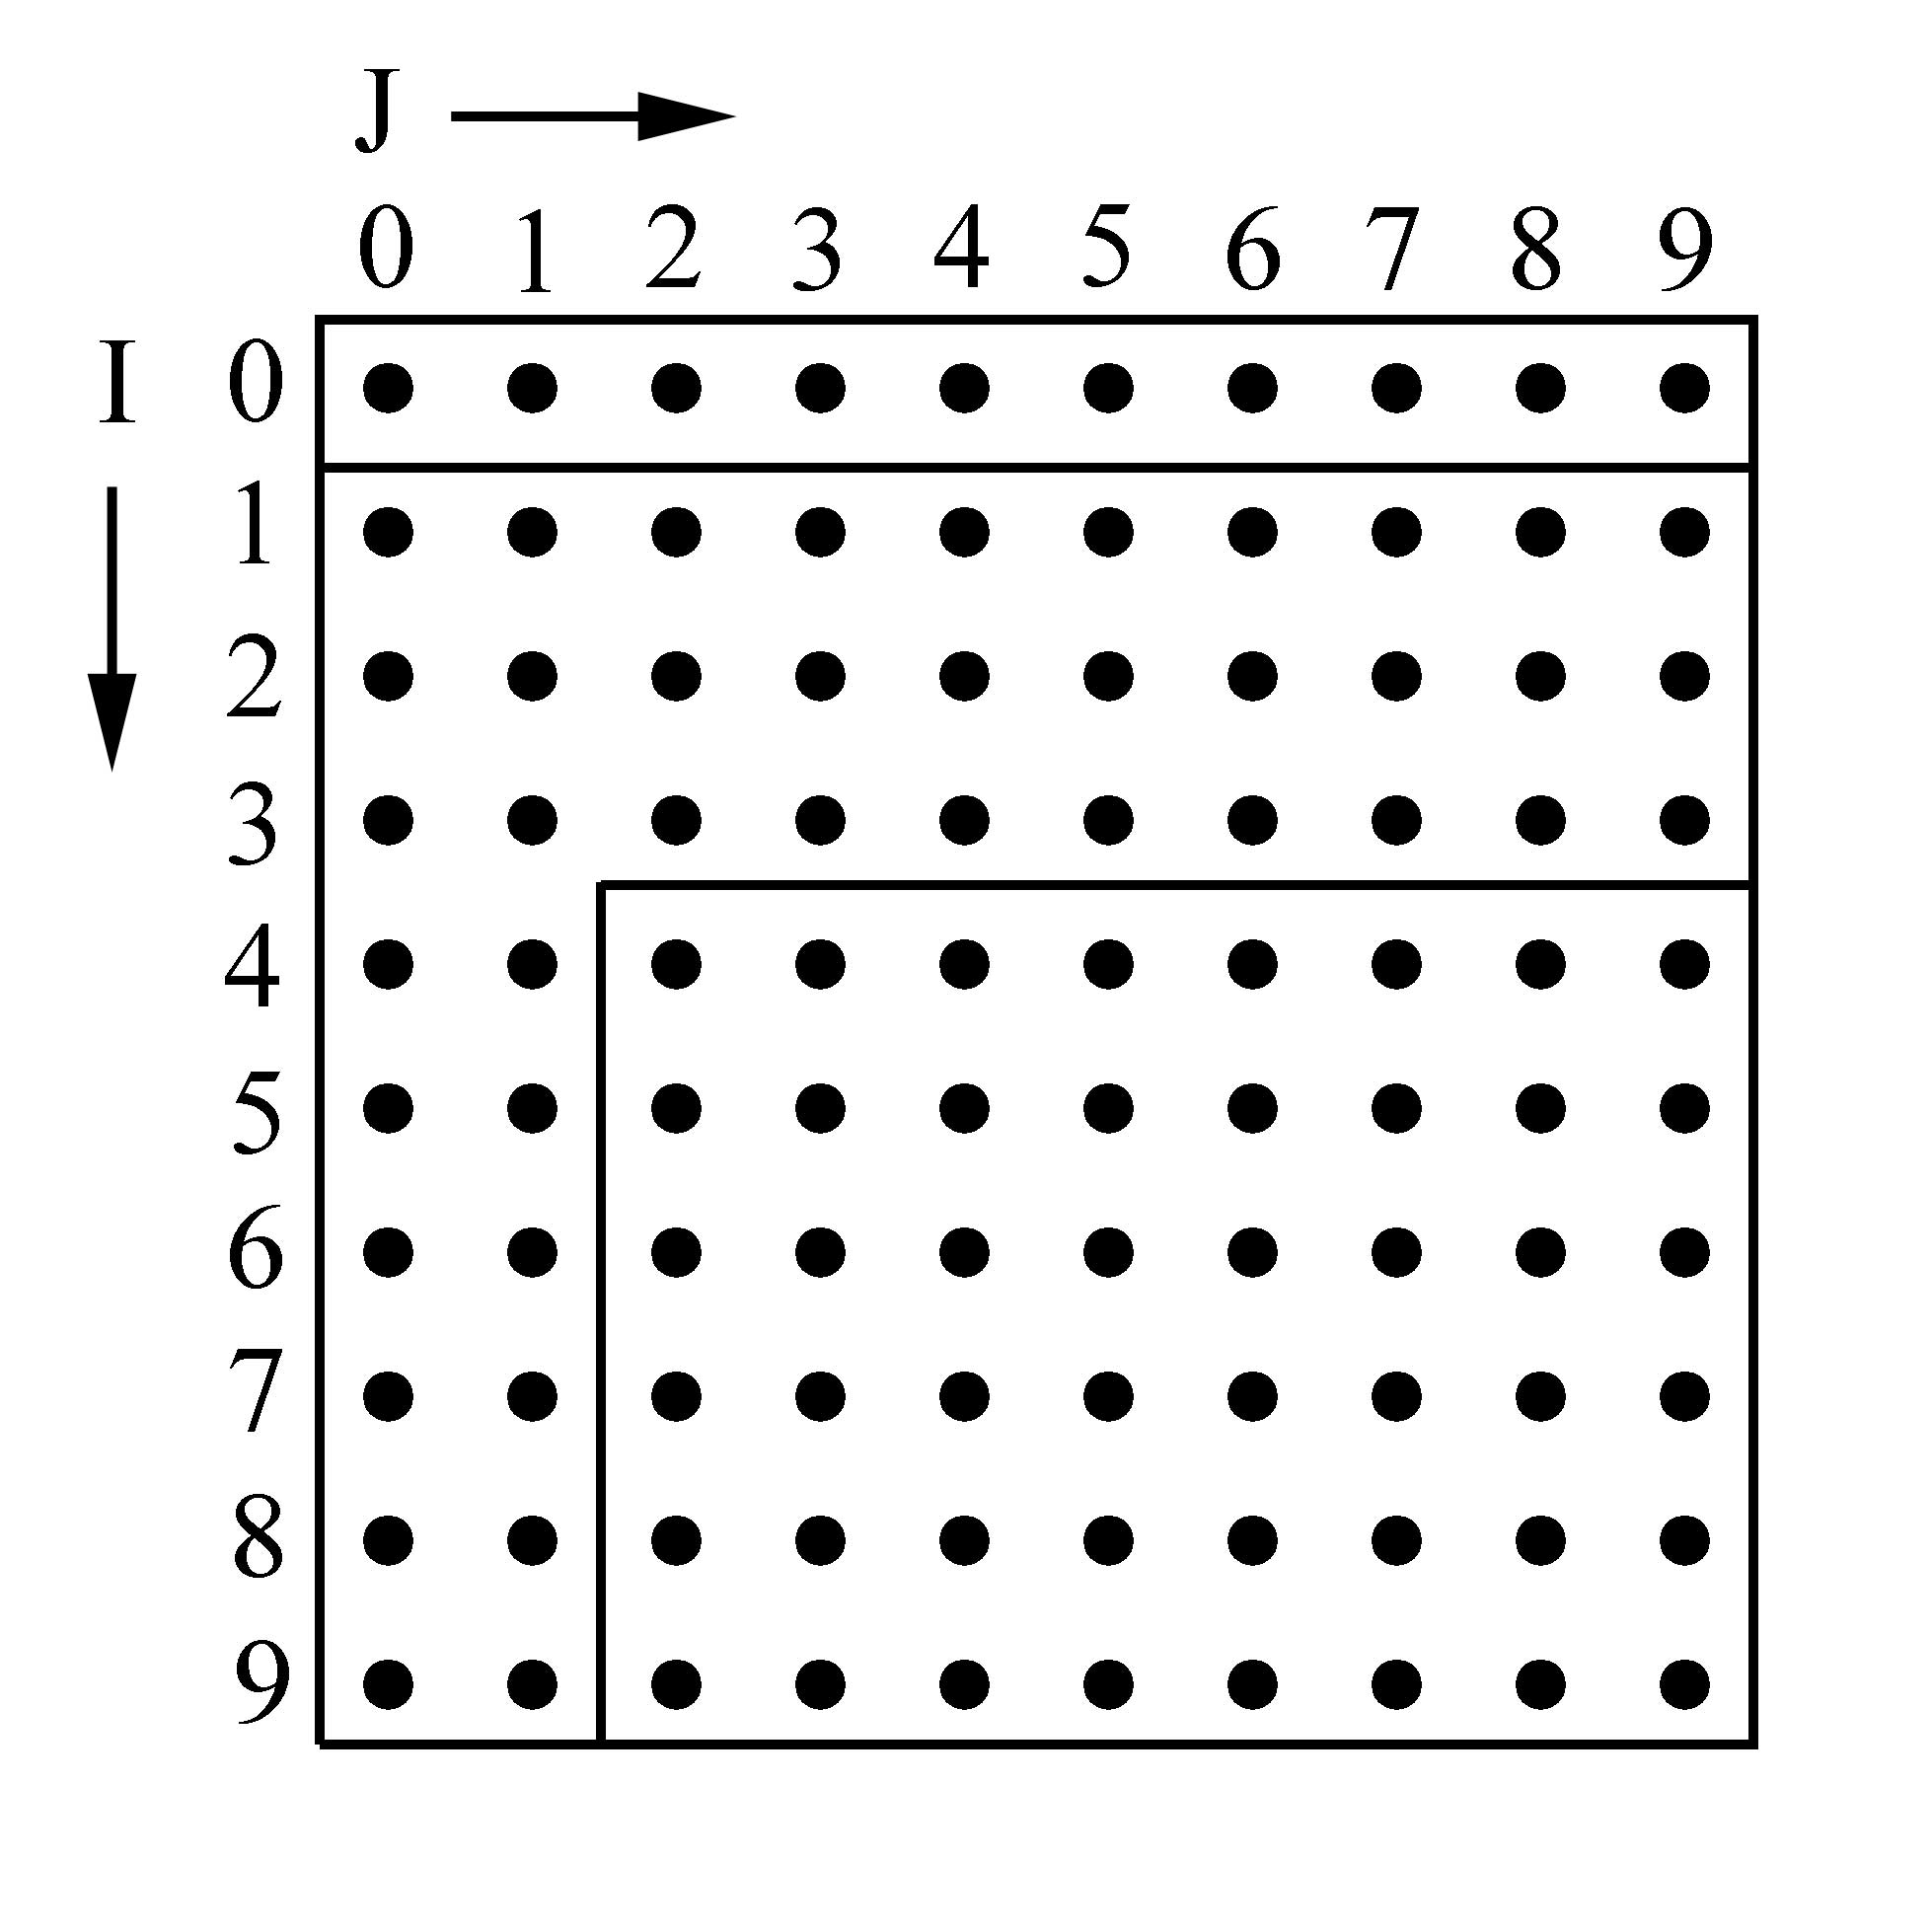
\includegraphics[width=0.5\textwidth]{Figures/variable_eg.jpg}
\end{figure}